\documentclass[10pt,aspectratio=169]{beamer}
% \documentclass[10pt,aspectratio=169,handout]{beamer}

% silence some Metropolis warnings
\usepackage{silence}
\WarningFilter{beamerthememetropolis}{You need to compile with XeLaTeX or LuaLaTeX}
\WarningFilter{latexfont}{Font shape}
\WarningFilter{latexfont}{Some font}

% define custom colors
\definecolor{dark gray}{HTML}{444444}
\definecolor{light gray}{HTML}{777777}
\definecolor{dark red}{HTML}{BB0000}
\definecolor{dark green}{HTML}{00BB00}

% configure metropolis
\usetheme[numbering=fraction]{metropolis}
\setbeamercolor{background canvas}{bg=white}
\setbeamercolor{frametitle}{bg=dark gray}
\setbeamercolor{alerted text}{fg=dark red}
\setbeamercolor{item projected}{bg=dark red}
\setbeamercolor{local structure}{fg=dark red}
\setbeamersize{text margin left=0.5cm,text margin right=0.5cm}
\setbeamercovered{transparent=10}

% use thicker lines
\makeatletter
\setlength{\metropolis@titleseparator@linewidth}{1pt}
\setlength{\metropolis@progressonsectionpage@linewidth}{1pt}
\makeatother

% custom bullet points
\setbeamertemplate{itemize item}{\color{dark red}$\blacktriangleright$}
\setbeamertemplate{itemize subitem}{\color{dark red}$\blacktriangleright$}
\setbeamertemplate{itemize subsubitem}{\color{dark red}$\blacktriangleright$}
\newcommand{\custombullet}{{\color{dark red}$\blacktriangleright$}\hspace{0.5em}}

% use classic font for math
\usefonttheme[onlymath]{serif}

% imports
\usepackage[english]{babel}
\usepackage[utf8]{inputenc}
\usepackage{amsthm}
\usepackage{amssymb}
\usepackage{amsmath}
\usepackage{amsfonts}
\usepackage{mathtools}
\usepackage{mathabx}
\usepackage{stmaryrd}
\usepackage{graphicx}
\usepackage{hyperref}
\usepackage{xfrac}
\usepackage{appendixnumberbeamer}

% check and x marks
\usepackage{pifont}
\newcommand{\cmark}{{\color{dark green}\ding{51}}\hspace{0.3em}}
\newcommand{\xmark}{{\color{dark red}\ding{55}}\hspace{0.5em}}

% diagrams
\usepackage{tikz}
\usetikzlibrary{decorations.pathreplacing}

% references
\usepackage[natbibapa]{apacite}
\bibliographystyle{apacite}
\renewcommand{\bibsection}{}

% use ampersands instead of "and" for text citations
\AtBeginDocument{\renewcommand{\BBAB}{\&}}

% possessive cites
\makeatletter
\patchcmd{\NAT@test}{\else \NAT@nm}{\else \NAT@nmfmt{\NAT@nm}}{}{}
\DeclareRobustCommand\citepos
  {\begingroup
   \let\NAT@nmfmt\NAT@posfmt
   \NAT@swafalse\let\NAT@ctype\z@\NAT@partrue
   \@ifstar{\NAT@fulltrue\NAT@citetp}{\NAT@fullfalse\NAT@citetp}}
\let\NAT@orig@nmfmt\NAT@nmfmt
\def\NAT@posfmt#1{\NAT@orig@nmfmt{#1's}}
\makeatother

% spaced-out lists
\newenvironment{wideitemize}{\itemize\addtolength{\itemsep}{10pt}}{\enditemize}
\newenvironment{wideenumerate}{\enumerate\addtolength{\itemsep}{10pt}}{\endenumerate}

% replace footnotes with buttons
\usepackage[absolute,overlay]{textpos}
\newcounter{beamerpausessave}
\newcommand{\always}[1]{
    \setcounter{beamerpausessave}{\value{beamerpauses}}
    \setcounter{beamerpauses}{0}
    \pause
    #1 
    \setcounter{beamerpauses}{\value{beamerpausessave}}
    \addtocounter{beamerpauses}{-1}
    \pause
}
\newcommand{\buttons}[1]{\always{
    \begin{textblock*}{\paperwidth}(0.015\textwidth, 1.022\textheight)
        \scriptsize
        #1
    \end{textblock*}
}}
\newcommand{\appendixbuttons}[1]{\always{
    \begin{textblock*}{\paperwidth}(0.015\textwidth, 1.043\textheight)
        \scriptsize
        #1
    \end{textblock*}
}}
\newcommand{\goto}[2]{\hyperlink{#1}{{\color{dark red}$\smalltriangleright$} #2}\hspace{0.5em}}
\newcommand{\goback}[2]{\hyperlink{#1}{{\color{dark red}$\smalltriangleleft$} #2}\hspace{0.5em}}

% custom appendix
\renewcommand{\appendixname}{\texorpdfstring{\translate{Appendix}}{Appendix}}

% change color of cites and URLs
\let\oldcite\cite
\let\oldcitet\citet
\let\oldcitep\citep
\let\oldcitepos\citepos
\let\oldcitetalias\citetalias
\let\oldcitepalias\citepalias
\let\oldurl\url
\def\cite#1#{\citeaux{#1}}
\def\citet#1#{\citetaux{#1}}
\def\citep#1#{\citepaux{#1}}
\def\citepos#1#{\citeposaux{#1}}
\def\citetalias#1#{\citetaliasaux{#1}}
\def\citepalias#1#{\citepaliasaux{#1}}
\def\url#1#{\urlaux{#1}}
\newcommand*\citeaux[2]{{\color{light gray}\oldcite#1{#2}}}
\newcommand*\citetaux[2]{{\color{light gray}\oldcitet#1{#2}}}
\newcommand*\citepaux[2]{{\color{light gray}\oldcitep#1{#2}}}
\newcommand*\urlaux[2]{{\color{light gray}\oldurl#1{#2}}}
\newcommand*\citeposaux[2]{{\color{light gray}\oldcitepos#1{#2}}}
\newcommand*\citetaliasaux[2]{{\color{light gray}\oldcitetalias#1{#2}}}
\newcommand*\citepaliasaux[2]{{\color{light gray}\oldcitepalias#1{#2}}}

% custom math commands
\DeclareMathOperator*{\argmax}{argmax}
\DeclareMathOperator*{\argmin}{argmin}
\renewcommand{\Pr}{\mathbb{P}}
\newcommand{\E}{\mathbb{E}}
\newcommand{\Var}{\mathbb{V}}
\newcommand{\Cov}{\mathbb{C}}
\newcommand{\overbar}[1]{\mkern 1.5mu\overline{\mkern-1.5mu#1\mkern-1.5mu}\mkern 1.5mu}

% tables
\usepackage{booktabs}
\usepackage{colortbl}
\usepackage{multirow}
\usepackage{makecell}
\arrayrulecolor{dark red}

% custom date
\usepackage{datetime}
\newdateformat{monthyeardate}{\monthname[\THEMONTH] \THEYEAR}

% fix pauses with graphics
\usepackage{fixpauseincludegraphics}


\usepackage{lipsum}
\usepackage{amsmath} 
\usepackage{amsthm} 
\usepackage{amssymb} 
\usepackage{mathtools}
%\usepackage{natbib}
\usepackage{dutchcal}


\newcommand{\vect}[1]{\boldsymbol{\mathbf{#1}}}
\newcommand{\pd}[2]{\frac{\partial{#1}}{\partial{#2}}}
\newcommand{\expect}[2]{\mathbb{E}_{#1}\left[{#2}\right]}
\newcommand{\expectsmall}[2]{\mathbb{E}_{#1}{#2}}
\newcommand{\expectsuper}[3]{\mathbb{E}_{#1}^{#2}\left[{#3}\right]}
\newcommand{\ind}[1]{\mathbbm{1}\left\{{#1}\right\}}
\newcommand{\prob}[1]{\mathbb{P}\left\{{#1}\right\}}
\newcommand{\derivative}[2]{\frac{d{#2}}{d{#1}}}
\newcommand{\cat}[1]{\citeasnoun{#1}}


% Bars for vectors
\newcommand*{\vertbar}{\rule[-1ex]{0.5pt}{2.5ex}}
\newcommand*{\horzbar}{\rule[.5ex]{2.5ex}{0.5pt}}


% title page
\title{Horizontal Merger Simulation and Multiproduct Demand Estimation}
\author{Chris Conlon}
\institute{NYU Stern and NBER}

\date{Summer 2023}




\begin{document}



%--------------
% TITLE PAGE
\begin{frame}[plain] %
\titlepage
\end{frame}


\begin{frame}{Who am I?}
I am an IO economist at NYU Stern School of Business, some work of mine:
\begin{itemize}
    \item Does \alert{common ownership} manifest in higher prices for consumer packaged goods? How much as common ownership grown in the US since 1980? What is the driver? (with Matt Backus and Mike Sinkinson)
    \item Can dominant firms use \alert{loyalty rebate contracts to exclude} more efficient rivals? (with Julie Mortimer)
    \item Why is market power a bad way to address \alert{externalities}? (with Nirupama Rao)
\item What are most effective ways to estimate multi-product demand systems? Including with micro data (with Jeff Gortmaker)
\item Do do \alert{different interventions} (price changes, quality reduction, second-choices) lead us to estimate different \alert{diversion ratios}? (with Julie Mortimer)
\item Can we flexibly estimate parameters with only aggregate data on market shares and some second-choice data? and some price-cost margins? (w/ Julie Mortimer and Paul Sarkis)
\end{itemize}
Not talking about first three today...
\end{frame}


\section{First: Some Review}


\begin{frame}{Cournot Model (1838) / Nash in Quantities}
Firms simultaneously choose $q_f$ to maximize profits and calculate FOC's where $Q=\sum_{f=1}^N q_f$ the total output of the industry.
\begin{align*}
\pi_i(q_f) &= P(Q)\cdot q_f - C_f(q_f)\\
\frac{\partial \pi_i(q_f)}{\partial q_f} &= (P(Q) - C_f'(q_f))  +  q_f  \cdot P'(Q) \cdot \frac{\partial Q}{\partial q_f}  = 0
\end{align*}
Cournot competition implies that $\frac{\partial Q}{\partial q_f} = 1$ and $\frac{\partial q_g}{\partial q_f} = 0$ for $f \neq g$.
\begin{align*}
\underbrace{P(Q) + \overbrace{P'(Q) \cdot q_f}}^{\text{\alert{Cournot Distortion}}}_{MR} =  mc_f
\end{align*}
We have that $\frac{q_f}{Q} \cdot \frac{\partial Q}{\partial q_f} = \frac{q_f}{\sum_{g=1}^n q_g} \equiv s_f$ or \alert{market share}.
\end{frame}




\begin{frame}{Asymmetric Cournot and HHI}
\begin{itemize}
\item The Cournot markup / Lerner Index is just:
\begin{align*}
\frac{P-mc_f}{P} &= \frac{s_f}{|\epsilon_D|}\\
\sum_{f=1}^N \frac{P - mc_f}{P} s_f &= \sum_{f=1}^n \frac{s_f^2}{|\epsilon_D|}
\end{align*}
\item Cournot: markups are proportional to market-share.
\item Obviously this nests symmetric case where $q_f = \frac{Q}{n}$ or $s_i = \frac{1}{n}$.
\item $HHI = \sum_f s_f^2$ is proportional to the \alert{share-weighted average markup}.
\item Can also work backwards form HHI to get effective ``number of firms''.
\item Here HHI is in units of $[0,1]$ instead of $[0,10000]$.
\begin{align*}
HHI = \sum_{i=1}^N s_i^2 = \frac{1}{n^*} \rightarrow n^{*} = \frac{1}{HHI}.
\end{align*}
\end{itemize}
\end{frame}



\begin{frame}{HHI and Welfare}
Under Cournot (and only Cournot) with constant MC, we can relate $HHI$ to particular measures of welfare:
\begin{itemize}
\item Cowling Waterson (1976) relate $HHI$ to producer share of revenue:
\begin{align*}
HHI =  \epsilon_d \cdot \frac{PS}{R}
\end{align*}
\item Spiegel (2020) relates $HHI$ to producer share of surplus:
\begin{align*}
HHI &=  \frac{1}{\epsilon_d \left(Q^{*}\right)} \cdot \frac{PS}{CS}\\
\frac{C S}{TS} &=\frac{1}{1+\epsilon_d \left(Q^{*}\right) \cdot HHI}
\end{align*}
\end{itemize}
\end{frame}




\begin{frame}{Cournot: Discussion}

\begin{itemize}
\item DOJ/FTC describe markets as:
\begin{itemize}
\item Highly Concentrated: $HHI \geq 2500$ (4 firms)
\item Moderately Concentrated: $HHI \in [1500,2500]$. $\Delta HHI \geq 250$ merits scrutiny.
\item Un-Concentrated: $HHI \leq 1500$. ($>6$ firms)
\end{itemize}
\item This has been important aspect of US HMG since 1980.
\item But this makes \alert{market share} or \alert{market definiton} high stakes
\item Whole Foods Case (2007)
\begin{itemize}
\item FTC alleges 2:1 merger for ``premium natural organic supermarket''
\item Merging parties argue they have combined market share less than 2\% of supermarket market.
\item Do we want cases to hinge on merging parties or whether or not Wal-Mart and Amazon are ``in market''?
\end{itemize}
\end{itemize}
\end{frame}



\begin{frame}{Multiproduct (Asymmetric) Bertrand}
\small
Consider the multi-product Bertrand problem where firms solve: $\arg \max_{p \in \mathcal{J}_f} \pi_f (\mathbf{p}) = \sum_{j \in \mathcal{J}_f} (p_j - c_j) \cdot q_j(\mathbf{p})$:
\begin{align*}
 0&= q_j(\mathbf{p}) + \sum_{k \in \mathcal{J}_f} (p_k - c_k) \frac{\partial q_{k}}{\partial p_j}(\mathbf{p}) \\
\rightarrow p_j &=q_{j}(\mathbf{p}) \left[-\frac{\partial q_{j}}{\partial p_{j}}(\mathbf{p})\right]^{-1} + c_{j} + \sum_{k \in \mathcal{J}_{f} \setminus j} \left(p_{k}-c_{k}\right) \underbrace{\frac{\partial q_{k}}{\partial p_{j}}(\mathbf{p})\left[-\frac{\partial q_{j}}{\partial p_{j}}(\mathbf{p})\right]^{-1}}_{D_{jk}(\mathbf{p})}\\
p_j(p_{-j}) &= \underbrace{\frac{1}{1+1/\epsilon_{jj}(\mathbf{p})}}_{\text{Markup}} \left[ c_j + \sum_{k \in \mathcal{J}_{f} \setminus j}  (p_k-c_k) \cdot  D_{jk} (\mathbf{p}) \right]\\
\underbrace{p_j\cdot\left(1+1/\epsilon_{jj}(\mathbf{p})\right)}_{\text{MR}} &=  c_j + \sum_{k \in \mathcal{J}_{f} \setminus j}  (p_k-c_k) \cdot  D_{jk} (\mathbf{p})
\end{align*}
We call $D_{jk}(\mathbf{p}) = \frac{\frac{\partial q_{k}}{\partial p_j}(\mathbf{p})}{\left| \frac{\partial q_{j}}{\partial p_j}(\mathbf{p}) \right|}$ the \alert{diversion ratio} and $\epsilon_{jj}$ the \alert{own elasticity} and these are the main deliverables.
\end{frame}




\begin{frame}[plain]
\frametitle{In Matrix/Vector Form}
\begin{align*}
q_j(\mathbf{p}) + \sum_{k \in \mathcal{J}_f} (p_k - c_k) \frac{\partial q_{k}}{\partial p_j}(\mathbf{p}) =0
\end{align*}

It is helpful to define the \alert{demand derivatives} $\Delta_{(j,k)}(\mathbf{p})  = - \frac{\partial q_{j}}{\partial p_k}(\mathbf{p})$ and the \alert{ownership matrix}:
\begin{align*}
\mathcal{H}_{(j,k)} = \left\{\begin{array}{lr}
          1 & \text{for }  (j,k) \in \mathcal{J}_f \text{ for any } f \\ 
      0 & \text{o.w}\\
        \end{array} \right\}
\end{align*}
We can re-write the FOC in matrix form where $\odot$ denotes Hadamard product (element-wise):
\begin{align*}
        \mathbf{q}(\mathbf{p}) &= (\mathcal{H} \odot \Delta(\mathbf{p})) \cdot (\mathbf{p} - \mathbf{mc}), \\
       \mathbf{mc} &=  \mathbf{p} - \underbrace{(\mathcal{H} \odot \Delta(\mathbf{p}))^{-1} \mathbf{q}(\mathbf{p})}_{\eta(\mathbf{p},\mathbf{q},\theta_2)}.
\end{align*}
Solving this is easy (just inverting a matrix).
\end{frame}


\begin{frame}
\frametitle{Unilateral Effects: What do mergers do?}
Change the owenrship matrix !
\begin{align*}
\underbrace{p_j\cdot\left(1+1/\epsilon_{jj}(\mathbf{p})\right)}_{\text{MR}} &=  c_j + \sum_{k \in \mathcal{J}_{f} \setminus j}  (p_k-c_k) \cdot  D_{jk} (\mathbf{p})
\end{align*}
\begin{itemize}
    \item \alert{Upward Pricing Pressure}: how does RHS change?
     $$UPP_j = \Delta c_j + \sum_{k \in \mathcal{J}_{g}}  (p_k-c_k) \cdot  D_{jk} (\mathbf{p})$$
     \item This tells us whether or not \alert{opportunity costs} increase/decrease?
     \item To get price predictions we have to solve $J$ equations and $J$ unknowns $\mathbf{p}$.
     \begin{itemize}
        \item Need to know $\frac{\partial \mathbf{p}}{\partial \mathbf{c}}$ (pass-through matrix).
    \end{itemize}
    \item What do we miss? \alert{Coordinated Effects}, \alert{Dynamics}, \alert{Innovation}, etc.
\end{itemize}
\end{frame}



\begin{frame}
\frametitle{Merger Simulation}
What does a merger do? \alert{change the ownership matrix}.
\begin{itemize}

\item Step 1: Recover marginal costs $\widehat{\mathbf{mc}} = \mathbf{p} +(\mathcal{H} \odot \Delta(\mathbf{p}))^{-1} \mathbf{q}(\mathbf{p})$.
\item Step 1a: (Possibly) adjust marginal cost $\widehat{\mathbf{mc}}\cdot (1-e)$ with some cost efficiency $e$.
\item Step 2: Change the ownership matrix $\mathcal{H}^{pre} \rightarrow \mathcal{H}^{post}$.
\item Step 3: Solve for $\mathbf{p}^{post}$ via: $\mathbf{p} = \widehat{\mathbf{mc}} - \Delta(\mathbf{p})^{-1}q(\mathbf{p})$.
\end{itemize}
\pause
\vspace{0.5cm}
\begin{itemize}
\item The first step is easy (just a matrix inverse).
\item The second step is trivial.
\item The third step is tricky because we have to solve an implicit system of equations. $\mathbf{p}$ is on both sides. (It turns out it isn't a contraction).
\end{itemize}
\end{frame}



\begin{frame}{Solution Methods}
How do we solve: $\mathbf{p} = \widehat{\mathbf{mc}} - \Delta(\mathbf{p})^{-1}q(\mathbf{p})$?
\begin{enumerate}
\item Gauss Jacobi: Simultaneous Best Reply  $p_j^{k+1}(\mathbf{p_{-j}^k})$.
\item Gauss Seidel: Iterated Best Response  $p_j^{k+1}(\mathbf{p_{<j}^{k+1}},\mathbf{p_{>j}^{k}})$.
\item Newton's Method: Set $\mathbf{p} - \widehat{\mathbf{mc}} + \Delta(\mathbf{p})^{-1}q(\mathbf{p})=0$\\ but requires derivatives of $\Delta(\mathbf{p})^{-1}q(\mathbf{p})$
\item Fixed point iteration: $\mathbf{p} \mapsfrom \widehat{\mathbf{mc}} - \Delta(\mathbf{p})^{-1}q(\mathbf{p})$
\begin{itemize}
\item Turns out this is \alert{not a contraction}.
\item But you can get lucky... $\mathbf{p} - \widehat{\mathbf{mc}} + \Delta(\mathbf{p})^{-1}q(\mathbf{p})=0$ means you have satisfied FOC's
\end{itemize}
\item Alternative fixed point.
\end{enumerate}
\end{frame} 

\begin{frame}{Exploit the logit formula}
For the logit the $\Delta$ matrix (for a single market) looks like:
\begin{align*}
\Delta_{(j,k)}(\mathbf{p}) = \left\{\begin{array}{lr}
       \int \alpha_i \cdot s_{ij}\cdot (1-s_{ij}) \, \partial F_i& \text{ if } j=k \\
          \quad -\int \alpha_i \cdot s_{ij} \cdot s_{ik} \, \partial F_i &  \text{ if }  j\neq k 
        \end{array} \right\}
\end{align*}
Which we can factor into two parts (for plain logit):
\begin{align*}
\Delta(\mathbf{p}) =  \underbrace{\text{ Diag}\left[ \alpha \, \mathbf{s}(\mathbf{p}) \, \right]}_{\Lambda(\mathbf{p})} -  \underbrace{\alpha \cdot \mathbf{s}(\mathbf{p}) \mathbf{s}(\mathbf{p})'}_{\Gamma(\mathbf{p})}
\end{align*}
$\Gamma(\mathbf{p})$ and $\Lambda(\mathbf{p})$ are $J \times J$ matrices and $\Lambda(\mathbf{p})$ is diagonal and $(j,k)$ is nonzero in $\Gamma(\mathbf{p})$ only if $(j,k)$ share an owner.
\end{frame}


\begin{frame}{Morrow Skerlos (2010) Fixed Point}
\begin{itemize}
\item After factoring we can rescale by $\Lambda^{-1} (\mathbf{p})$
\begin{align*}
(\mathbf{p}-\mathbf{mc} ) \mapsfrom \Lambda^{-1}(\mathbf{p}) \cdot \Gamma(\mathbf{p})\cdot(\mathbf{p}- \mathbf{mc}) - \Lambda^{-1}(\mathbf{p})\cdot s(\mathbf{p})
\end{align*}
\item This alternative fixed point is in fact a contraction.
\item Moreover the rate of convergence is generally fast and stable (much more than Gauss-Seidel or Gauss-Jacobi).
\item Honestly, this is the best way to solve large pricing games. It nearly always wins and doesn't require derivatives.
\item Coincidentally, this is what \texttt{PyBLP} defaults to.
\end{itemize}
\end{frame}



% \begin{frame}
% \frametitle{Starting Point: McFadden and MLE}
% Each individual's choice $d_{ij} \in\{0,1\}$ and $\sum_{j \in \mathcal{J}} d_{ij} =1$.\\
% Consumers make mutually exclusive and exhaustive choices to maximize (indirect) utility:
% \begin{align*}
% u_{ij} &= \beta_i \, x_{ij}  + \varepsilon_{ij} \text{ and }
% u_{i0} = \varepsilon_{i0}\\
% d_{ij} &=1 \text{ IFF } [u_{ij} > u_{ik}\, \forall k \neq j]
% \end{align*}
% Choices follow a Categorical distribution:
% \begin{align*}
% (d_{i1},\ldots,d_{iJ},d_{i0}) \sim \text{Categorical} (s_{i1},\ldots,s_{iJ},s_{i0} ) 
% \end{align*}
% \end{frame}


% \begin{frame}
% \frametitle{Starting Point: McFadden and MLE}
% If we assume that $\varepsilon_{ij}$ is Type I extreme value and $\beta_{\iota} \sim f(\beta_{\iota} \mid \theta)$ (some known parametric distribution) then we can write:
% \begin{align*}
% s_{ij}(\theta)= \mathbb{P}(d_{ij}=1) = \int \frac{\exp[\beta_{\iota} \, x_j]}{1+\sum_{k \in \mathcal{J}} \exp[\beta_{\iota} \, x_k]}\, f(\beta_{\iota} \mid \theta)\, \partial \beta_{\iota}
% \end{align*}
% Which gives us the log-likelihood:
%  \begin{align*}
%  \ell(\theta) = \sum_{i=1}^N \sum_{j \in \mathcal{J} \cup \{0\}} d_{ij} \log s_{ij}(\mathbf{x_i} \mid \theta)
%  \end{align*}
%  There are a bunch of challenges, not least among which is that the above is \alert{inconsistent} if the integral is evaluated with error that doesn't decrease in $N$.
% \end{frame}







% \begin{frame}
% \frametitle{Starting Point: Moving to Aggregate Data}
% If each individual is \alert{exchangable} then ex-ante they have the same choice probabilities: $s_{ij}=s_j$, and the sum of $M$ Categoricals is Multinomial:
% \begin{align*}
% (q_{1}^{*},\ldots,q_{J}^{*},q_{0}^{*}) \sim \text{Mult} (M, s_{1},\ldots,s_{J},s_{0} ) 
% \end{align*}
% where $q_{j}^{*}=\sum_{i=1}^M d_{ij}$ is a \alert{sufficient statistic}. 
% \begin{itemize}
% \item If $M$ gets large enough then $(\frac{q_1}{M},\ldots,\frac{q_J}{M},\frac{q_0}{M})\rightarrow (\mathfrak{s}_1,\ldots,\mathfrak{s}_J,\mathfrak{s}_0)$
%  \item Idea: Equate observed market shares to the conditional choice probabilities $(s_1(\mathbf{x_i},\theta),\ldots,s_J(\mathbf{x_i},\theta),s_0(\mathbf{x_i},\theta))$.
% \item  Challenges: We probably don't really observe $q_0$ and hence $M$.
% \item Introduce idea of market $t$ (otherwise not much data!)
% \end{itemize}
% \end{frame}




% \begin{frame}\frametitle{Lots of papers stop here}
% \begin{columns}
% \begin{column}{0.3\textwidth}
%      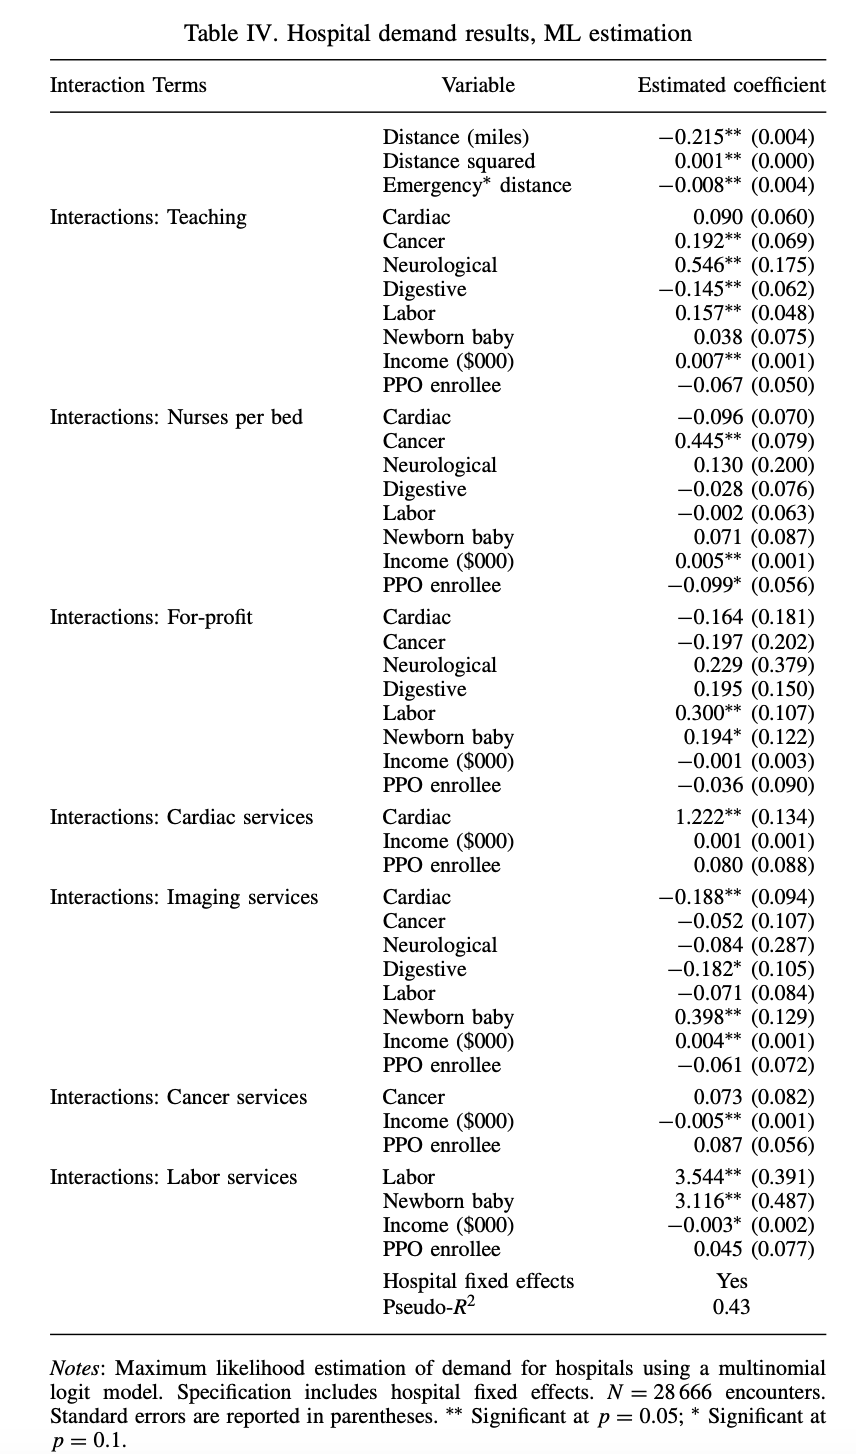
\includegraphics[height=\textheight]{resources/ho_2006}      
% \end{column}
% \begin{column}{0.7\textwidth}
% \begin{itemize}
% \item This just MLE on the full individual data from Ho (2006)
% \begin{itemize}
% \item There is no unobserved heterogeneity, just a deterministic $\beta(y_i)$ where $y_i$ are demographics.
% \end{itemize}
% \item The ``FTC model'' (Raval, Rosenbaum, Wilson RJE 2022)/ (Raval, Rosenbaum, Tenn EI 2017) groups individuals by income, diagnosis, and zip code and estimates a separate set of $\beta_{g(i)}$ for each group.
% \item Hopsitals are a bit special: distance $x_{ij}$ does much of the work (special regressor)
% \item Price endogeneity not really a concern (?)
% \end{itemize}
% \end{column}
% \end{columns}
% \end{frame}

% \begin{frame}{Semiparametric Extensions: Fox Kim Ryan Bajari (QE 2011)}
% \vspace{-0.5cm}
% \begin{align*}
% \nonumber \min_{\pi_i} \sum_{j,t} \left(\mathcal{S}_{jt}(\mathbf{x_t}) - \sum_i \pi_i \cdot s^{*}_{ijt}(\beta^{*}_i, \mathbf{x_t})\right)^2 &
% \quad \text{subject to} \quad s^{*}_{ijt}(\beta^{*}_i, \mathbf{x_t}) = \frac{e^{\beta^{*}_i x_{jt} }}{1+\sum_{j'}e^{\beta^{*}_i x_{j't}}}\\
%    0\leq  \pi_i \leq 1,& \quad   \sum_i \pi_i = 1
% \end{align*}
% \vspace{-0.5cm}
% \begin{enumerate} 
%     \item Draw a large number (thousands?) of $(\beta^{*}_i$ from a prior distribution $g(\beta_i)$ more dispersed than the true $f(\beta_i)$
%     \item Compute individual choice probabilities $ s^{*}_{ijt}(\beta^{*}_i)$
%     \item Estimate above by constrained least squares (non-negative lasso)
%     \item This produces sparse models. (most $\pi_i=0$)
% \end{enumerate}
% Fixed coefficients require EM. See Heiss, Hetzenecker, Osterhaus (JE 2022) for details (and elastic net variant $\sum_i \pi_i^2 \leq t$).
% \end{frame}


% \begin{frame}{Applications of Fixed Grid Estimators}
% These estimators are helpful when computing choice probabilities is time-consuming (ie: when choices are dynamic). Some recent examples:
% \begin{itemize}
%     \item Nevo, Turner, Williams (ECMA 2016): Broadband competition
%     \item Blundell, Gowrisankaran, Langer (AER 2020): EPA regulation
% \end{itemize}
% \end{frame}







% % \begin{frame}

% % \end{frame}


% % \begin{frame}
% % \frametitle{Multinomial Logit: Estimation with Aggregate Data}
% % Now suppose we have aggregate data: $(q_1,\ldots,q_J,q_0)$ where $M = \sum_{j \in \mathcal{J}} q_j$.
% % \begin{itemize}
% % \item If $M$ gets large enough then $(\frac{q_1}{M},\ldots,\frac{q_J}{M},\frac{q_0}{M})\rightarrow (\mathfrak{s}_1,\ldots,\mathfrak{s}_J,\mathfrak{s}_0)$
% % \begin{itemize}
% % \item Idea: Observe $(\mathfrak{s}_1(\mathbf{x_i}),\ldots,\mathfrak{s}_J(\mathbf{x_i}), \mathfrak{s}_0(\mathbf{x_i}))$ without sampling variance.
% % \end{itemize}
% % \item Choose $\theta$ that minimizes distance: MLE? MSM? Least Squares? etc.
% % \end{itemize}
% % \end{frame}



\section*{Review: ``Classic'' BLP (1995) Models}

\begin{frame}
\frametitle{Demand: Product Space}
\begin{itemize}
    \item Remember we need $\epsilon_{jj}(\mathbf{p})$ and $D_{jk}(\mathbf{p}) = \frac{\epsilon_{jk}(\mathbf{p})}{\epsilon_{jj}(\mathbf{p})}\cdot \frac{q_j}{q_k}$ so $\epsilon_{jk}(\mathbf{p})$.
    \item Multiple ``markets'' $t$ with different prices/assortment.
    \item One approach might be \alert{constant elasticity} or \alert{log-log}
    \begin{align*}
        \log Q_{jt} = \beta_0 + \sum_{k} \beta_{j,k} \log P_{kt} + e_{jt}
    \end{align*}
    \item Even better might be \alert{Almost Ideal Demand} (Deaton Muellbauer 1980) or \alert{trans-log}
    \begin{align*}
        \log Q_{jt} = \beta_0 + \sum_{k} \beta_{j,k} \log P_{kt} + \sum_{k} \gamma_{j,k} \log P_{kt} \log P_{jt} +  e_{jt}
    \end{align*}
    \item Problem: If we have $J$ products, we need to estimate $J^2$ elasticities.
    \item Bigger Problem: every time $P_k$ shows up on RHS, we need an instrument (!)
\end{itemize}
\end{frame}

\begin{frame}
\frametitle{Demand: Product Space (Multinomial Probit)}

\begin{itemize}
    \item Assume consumers have unit demand and make discrete choices
    \item Label $j=0$ the no-purchase or outside option has $V_{i0t}=0$
    \begin{align*}
        u_{ijt} = V_{ijt} - \alpha p_{jt} +  \varepsilon_{ijt} \text{ with } \boldsymbol{\varepsilon_{it}} \sim \mathcal{N}(0,\Omega)
    \end{align*}
    \item Idea: calculate $\sigma_{ijt} = \mathbb{P}(u_{ijt} > u_{ikt} \text{ for all } k \neq j)$
    \item But some problems...
    \begin{itemize}
        \item Have to \alert{simulate draws from normals} to calculate $s_{ijt}$ (no closed form)
        \item Still have $J^2$ elements in $\Omega$ (Maybe more like $(J+1) \cdot J / 2$ with symmetry)
        \item Still need $J$ instruments.
    \end{itemize}

\end{itemize}
\end{frame}



\begin{frame}
\frametitle{Demand: Characteristic Space (Multinomial Logit)}

\begin{itemize}
    \item What if we assumed that products were just bundles of characteristics
    \item Assume that $V_{ijt} = x_{jt} \beta - \alpha p_{jt}$
    \item Also change the distribution of $\varepsilon_{ij}$ to be Type I EV (Gumbel/Logit)
    \begin{align*}
        u_{ijt} = x_{jt} \beta- \alpha p_{jt} +  \varepsilon_{ijt} \text{ with } \varepsilon_{ijt} \sim \text{IID Type I EV}.
    \end{align*}
    \item Now $\sigma_{jt}$ is easy to calculate (and doesn't depend on $i$)
     \begin{align*}
          \sigma_{jt} \equiv \mathbb{P}(u_{ijt} > u_{ikt} \text{ for all } k \neq j)  = 
    \frac{e^{x_{jt} \beta- \alpha p_{jt}}}{1+\sum_k e^{x_{kt} \beta- \alpha p_{kt} }}
    \end{align*}
    \item But now IV is hard: because $\mathbf{p_t}$ enters the model \alert{nonlinearly}
\end{itemize}
\end{frame}





\begin{frame}
\frametitle{Inversion: IIA Logit (Berry 1994)}
Add unobservable error for each $s_{jt}$ labeled $\alert{\xi_{jt}}$ and set\\
 \alert{observed shares} $\mathcal{S}_{jt} = \sigma_{j}(\boldsymbol{\delta_{t}},\alpha,\beta)$ \alert{predicted shares}.
\begin{align*}
u_{ijt} &= \underbrace{x_{jt} \beta -\alpha p_{jt} + \alert{\xi_{jt}}}_{\delta_{jt}} +  \varepsilon_{ijt} , \quad 
\sigma_j(\boldsymbol{\delta_{t}}) = \frac{e^{\delta_{jt}} }{1+\sum_k e^{\delta_{kt}} } \\
 \log \mathcal{S}_{jt} - \log \mathcal{S}_{0t} &= \delta_{jt} - \underbrace{\delta_{0t}}_{=0} 
 = x_{jt} \beta -\alpha p_{jt} + \xi_{jt}
\end{align*}
\vspace{-0.5cm}
\begin{itemize}
\item The idea is that $\alert{\xi_{jt}}$ is observed to the firm when prices are set, but not to us the econometricians.
\item Potentially correlated with price $\text{Corr}(\xi_{jt},p_{jt}) \neq 0$
\item But not characteristics $\mathbb{E}[\xi_{jt} \mid  x_{jt}]=0$.
\begin{itemize}
\item This allows for products $j$ to better than some other product in a way that is not fully explained by differences in $x_j$ and $x_k$.
\item Something about a BMW makes it better than a Peugeot but is not fully captured by characteristics that leads higher sales and/or higher prices.
\item Consumers agree on its value  (\alert{vertical component}).
\end{itemize}
\item This is just Linear IV!
\end{itemize}
\end{frame}


\begin{frame}
\frametitle{Multinomial Logit: Disadvantages}
\begin{itemize}
\item To set \alert{observed shares} $=$ \alert{predicted shares} we need \alert{large markets} (lots of people making decisions) otherwise we have \alert{measurement error} in shares.
\item The logit has some unfortunate properties:
\begin{itemize}
    \item $\epsilon_{jj} = \alpha \cdot p_j \cdot (1-s_j)$ (increasing in own price!)
    \item $\epsilon_{jk} = \alpha \cdot p_j \cdot s_k $ (doesn't depend on $s_j$!)
    \item IIA/Proportional substitution $\frac{s_j}{s_k}$ is unaffected by $x_{l}$
    \item IIA/Proportional substitution $D_{j \rightarrow k} = \frac{s_k}{1-s_j}$
\end{itemize}
\end{itemize}
\pause
But we can solve these with \alert{unobserved heterogeneity} or \alert{random effects}.
\begin{align*}
u_{ijt} &= \delta_{jt} +\mu_{ijt}(\theta_2) +  \varepsilon_{ijt}. 
\end{align*}
where $\mu_{ijt}$ is mean zero.
\end{frame}



\begin{frame}
\frametitle{What about Nested Logit?}
The most common solution allow for correlated preferences among products in the same nest
\begin{align*}
u_{ijt} &= \delta_{jt} +\eta_{i,g(j),t}(\rho) +  \varepsilon_{ijt}(\rho). 
\end{align*}
This model is only as good as our groupings $g(j)$.
\begin{itemize}
    \item We still get IIA/proportional substitution \alert{within nest}.
    \item Define: $Z\left(\rho, s_g\right)=\left[\rho+(1-\rho) s_g\right] \in(0,1]$
    \item For same group : $$ D_{j \rightarrow k}^*=\frac{s_{k \mid g}}{Z^{-1}\left(\rho, s_g\right)-s_{j \mid g}} $$
    \item For different groups : $$ D_{j \rightarrow k}^{**}=\frac{s_k(1-\rho)}{1-s_{j \mid g} \cdot Z\left(\rho, s_{g(j)}\right)} $$
\end{itemize}
This gets used a ton at DOJ/FTC (with all goods in one nest). Why?\\
\end{frame}


\begin{frame}
\frametitle{Inversion: Berry, Levinsohn, Pakes (1995)}
We can't solve for $\delta_{jt}$ directly this time
\begin{eqnarray*}
\sigma_j(\boldsymbol{\delta_t}; \mathbf{x_t}; \theta_2) &=& \int \frac{\exp[\delta_{jt} +  \mu_{ij} ]}{1+\sum_k \exp[\delta_{kt} + \mu_{ik} ]} f(\boldsymbol{\mu_i}| \widetilde{\theta_2})
\end{eqnarray*}
 \begin{itemize}
    \item We typically parametrize $\mu_{ijt} = x_{jt} \cdot [\Pi \, y_i + \Sigma \, \nu_{i}]$ where $y_i$ are demographics and $\nu_i$ are unobserved heterogeneity (typically multivariate normal).
    \item Label $\widetilde{\theta}_2 = [\Pi, \Sigma]$ and $\theta_2 =[\alpha, \widetilde{\theta}_2 ]$
 \item This is a $J \times J$ system of equations for each $t$.
 \item It is diagonally dominant.
 \item There is a unique vector $\xi_t$ that solves it for each market $t$.
 \end{itemize}
\end{frame}

\begin{frame}
\frametitle{Lots of ways to solve equations (Conlon Gortmaker 2020)}
 \begin{itemize}
     \item If you can work out $\frac{\partial \sigma_{jt}}{\partial \delta_{kt}}$ (easy) you can solve this using Newton's Method. 
 \item BLP prove (not easy) that this is a \alert{contraction mapping}.
\begin{eqnarray*}
    \boldsymbol{\delta^{(k)}}(\theta) = \boldsymbol{\delta^{(k-1)}}(\theta) + \log(\mathcal{S}_{j}) - \log(\sigma_{j}(\boldsymbol{\delta_t}^{(k-1)}, \theta)
\end{eqnarray*}

\begin{itemize} 
  \item Practical tip: $\epsilon_{tol}$ needs to be as small as possible. ($\approx 10^{-13}$).
 \item Practical tip: Contraction isn't as easy as it looks:  $ \log(\sigma_{j}(\delta_t^{(k-1)}, \theta)$ requires computing the numerical integral each time (either via quadrature or monte carlo).
\end{itemize}
\item We can use \alert{accelerated fixed point} techniques (SQUAREM) (see Reynaerts, Varadhan, and Nash 2012). [PyBLP default].
  \end{itemize}
 \end{frame}


 \begin{frame}
\frametitle{BLP Pseudocode}
\footnotesize
From the outside, in:
\begin{itemize}
\item Outer loop: search over nonlinear parameters $\theta$ to minimize GMM objective:
 \begin{eqnarray*}
 \widehat{\theta_{BLP}} = \arg \max_{\theta_2} (Z' \hat{\xi}(\theta_2)) W  (Z' \hat{\xi}(\theta_2))'
 \end{eqnarray*}
 \item Inner Loop:
 \begin{itemize}
% \item Fix $\theta$.
\item Solve for $\delta$ so that $\sigma_{jt}(\delta,\theta_2) = \tilde{S}_{jt}$.
\begin{itemize}
\item Computing $s_{jt}(\delta,\theta)$ requires numerical integration (quadrature or monte carlo).
\end{itemize}
 \item We can do IV-GMM to recover $\hat{\alpha}(\theta_2),\hat{\beta}(\theta_2),\hat{\xi}(\theta_2)$.
  \begin{eqnarray*}
\delta_{jt}= x_{jt} \beta -\alpha p_{jt}+  \xi_{jt}
 \end{eqnarray*}
  \item Use $\hat{\xi}(\theta_2)$ to construct moment conditions.
 \end{itemize}
 \item When we have found $\hat{\theta}_{BLP}$ we can use this to update $W \rightarrow W(\hat{\theta}_{BLP})$ and do 2-stage GMM.
 \end{itemize}
\end{frame}




 \begin{frame}
\frametitle{BLP Estimation}
The model is still defined by CMR $\mathbb{E}[\xi_{jt} \mid  z_{jt}^D]=0$
\begin{itemize}
 \item Now that you have done change of variables to get:
 \begin{eqnarray*}
\delta_{jt}= x_{jt} \beta -\alpha p_{jt}+  \xi_{jt}
 \end{eqnarray*}
 \item We can do IV-GMM to recover $\hat{\alpha}(\theta_2),\widehat{\beta}(\theta_2),\widehat{\xi}(\theta_2)$.
 \item Outer Loop update guess $\theta$, solve for $\delta$ and repeat.
 \begin{eqnarray*}
 \widehat{\theta_{BLP}} = \arg \max_{\theta} (Z' \widehat{\xi}(\theta_2)) W  (Z' \widehat{\xi}(\theta_2))'
 \end{eqnarray*}
 \item When we have found $\widehat{\theta_2}_{BLP}$ we can use this to update $W \rightarrow W(\widehat{\theta_2}_{BLP})$ and do 2-stage GMM.
 \end{itemize}
\end{frame}



\begin{frame}
\frametitle{BLP Extensions: Panel Data}
\begin{itemize}
\item with enough observations on the same product it is possible to include fixed effects
\begin{eqnarray*}
\delta_{jt}(\theta_2) = x_{jt} \beta - \alpha p_{jt} + \underbrace{\xi_{jt}}_{\xi_{j} + \xi_t + \Delta \xi_{jt}}
\end{eqnarray*}
\item What does $\xi_{j}$ mean in this context?
\item What would $\xi_t$ mean in this context?
\item $\Delta \xi_{jt}$ is now the structural error term, this changes our identification strategy a little. 
\begin{itemize}
\item Good: endogeneity problem less severe.
\item Bad: less variation in IV.
\end{itemize}
\end{itemize}
\end{frame}


\section{Adding Supply}
\begin{frame}{Supply}
\begin{itemize}
\item Economic theory gives us some additional powerful restrictions.
\item We may want to impose $MR = MC$.
\item Alternatively, we can ask -- what is a good instrument for demand? \alert{something from another equation} (ie: supply).
\end{itemize}
\end{frame}

\begin{frame}{Some setup}
We can break up the parameter space into three parts:
\begin{itemize}
\item $\theta_1$: linear exogenous demand parameters: $\beta$ 
 \item $\theta_2$: parameters including price and random coefficients (endogenous / nonlinear)
 \item $\theta_3$: linear exogenous supply parameters.
\end{itemize}
\end{frame}


\begin{frame}{Recovering Marginal Costs }
Recover implied markups/ marginal costs, and assume a functional form for $mc_{jt}(x_{jt},w_{jt})$.
\begin{align*}
\mathbf{mc}(\theta_2)&= \mathbf{p}- \boldsymbol{\eta}(\mathbf{p},\mathbf{s},\theta_2)\\
f(mc_{jt}) &= [\textrm{x}_{jt} \,, \textrm{w}_{jt}] \theta_3 + \omega_{jt}
\end{align*}
Which we can solve for $\omega_{jt}$:
\begin{align*}
\omega_{jt} &=  f(\mathbf{p}- \boldsymbol{\eta}(\mathbf{p},\mathbf{s},\theta_2) ) -[\textrm{x}_{jt} \,, \textrm{w}_{jt}] \theta_3 
\end{align*}
\begin{itemize}
\item $f(\cdot)$ is usually $\log(\cdot)$ or identity.
\item We can use this to form additional moments: $\E[\omega_{jt} \mid  z_{jt}^{s}]=0$.
\item We can just stack these up with the demand moments $E[\xi_{jt}' Z_{jt}^d]=0$.
%\item Now I have $\dim(Z^d) + \dim(Z^s)$ moments altogether.
\item This step is optional but can aid in identification (if you believe it).
\end{itemize}
\end{frame}


% \begin{frame}{Additional Details}
% Some different definitions:
% \begin{alignat}{3}
% \label{eq:stacked}
% \nonumber y_{jt}^D &:= \widehat \delta_{jt}(\theta_2) + \alpha p_{jt} &=(\textrm{x}_{jt} \-\ \textrm{v}_{jt})' \beta + \xi_t &=: x_{jt}^{D\prime}\beta + \xi_{jt} \\ 
% y_{jt}^S &:= \widehat{mc}_{jt}(\theta_2) &= (\textrm{x}_{jt} \-\ \textrm{w}_{jt})'\gamma + \omega_t &=: x_{jt}^{S\prime} \gamma + \omega_{jt} 
% \end{alignat}
% Stacking the system across observations yields:
% \begin{align}
% \underbrace{\begin{bmatrix} y_D \\ y_S \end{bmatrix}}_{2N\times1} = 
% \underbrace{\begin{bmatrix}
% X_D & 0 \\
% 0 & X_S 
% \end{bmatrix}}_{2N\times(K_1+K_3)}
% \underbrace{\begin{bmatrix}
% \beta \\ \gamma %\Gamma_D \\ \Gamma_S
% \end{bmatrix}}_{(K_1+K_3)\times1} + 
% \underbrace{\begin{bmatrix}
% \xi \\ \omega % \varepsilon_D \\ \varepsilon_S
% \end{bmatrix}}_{2N\times 1}
% \end{align}
% \end{frame}



\begin{frame}{Simultaneous Supply and Demand: in details}
\footnotesize
\begin{enumerate}[(a)]
\item For each market $t$: solve $\mathcal{S}_{jt} = \sigma_{jt}(\delta_{\cdot t},\theta_2)$ for $\widehat{\delta}_{\cdot t}(\theta_2)$.
\item For each market $t$: use $\widehat{\delta}_{\cdot t}(\theta_2)$ to construct $\eta_{\cdot 
t}(\mathbf{q_t},\mathbf{p_t},\widehat{\delta}_{\cdot t}(\theta_2),\theta_2)$
\item For each market $t$: Recover $\widehat{mc}_{jt}(\widehat{\delta}_{\cdot t}(\theta_2),\theta_2) = p_{jt} - \eta_{jt}(\widehat{\delta}_{\cdot t}(\theta_2),\theta_2)$
\item Stack up $\widehat{\delta}_{\cdot t}(\theta_2)$ and $\widehat{mc}_{jt}(\widehat{\delta}_{\cdot t}(\theta_2),\theta_2)$ and use linear IV-GMM to recover $[\widehat{\theta}_1(\theta_2), \widehat{\theta}_3(\theta_2) ]$ following the recipe in Appendix of Conlon Gortmaker (2020)
\item Construct the residuals:
\begin{align*}
\nonumber    \widehat{\xi}_{jt}(\theta_2) &= \widehat{\delta}_{jt}(\theta_2) -  x_{jt} \widehat{\beta}(\theta_2) + \alpha p_{jt}\\
    \widehat{\omega}_{jt}(\theta_2) &= \widehat{mc}_{jt}(\theta_2) -  [x_{jt}\, w_{jt}]\, \widehat{\gamma}(\theta_2)
\end{align*}
\item Construct sample moments
\begin{align*}
\nonumber g_n^D(\theta_2)=\frac{1}{N} \sum_{jt} Z_{jt}^{D\prime} \widehat{\xi}_{jt}(\theta_2)\\
 g_n^S(\theta_2)=\frac{1}{N} \sum_{jt} Z_{jt}^{S \prime} \widehat{\omega}_{jt}(\theta_2)
\end{align*}
\item Construct GMM objective $Q_n(\theta_2)= \left[ {\begin{array}{c} g_n^d(\theta_2) \\ g_n^s(\theta_2) \end{array} } \right]' W  \left[ {\begin{array}{c} g_n^d(\theta_2) \\ g_n^s(\theta_2) \end{array} } \right] $
\end{enumerate}
\end{frame}


\section{Micro Moments}

\begin{frame}{Micro BLP is used a lot}
    \vspace{0.5em}
    \scriptsize
    \begin{tabular}{rlrl}
        Paper & Industry & Paper & Industry \\
        \midrule
        \cite*{petrin2002quantifying} & Automobiles & \cite*{barwick2017local} & Automobiles \\
        \cite*{berry2004differentiated} & Automobiles & \cite*{murry2017advertising} & Automobiles \\
        \cite*{thomadsen2005effect} & Fast Food & \cite*{wollmann2018trucks} & Commercial Vehicles \\
        \cite*{goeree2008limited} & Personal Computers & \cite*{li2018better} & Automobiles \\
        \cite*{ciliberto2010public} & Cigarettes & \cite*{li2018empirical} & Digital Cameras \\
        \cite*{nakamura2010accounting} & Coffee & \cite*{backus2021common} & Cereal \\
        \cite*{beresteanu2011gasoline} & Automobiles & \cite*{grieco2021evolution} & Automobiles \\
        \cite*{li2012traffic} & Automobiles & \cite*{neilson2021targeted} & Primary Schools \\
        \cite*{copeland2014intertemporal} & Automobiles & \cite*{armitage2022regulatory} & Automobiles \\
        \cite*{starc2014insurer} & Health Insurance & \cite*{dopper2022rising} & Retail \\
        \cite*{ching2015quantifying} & Nursing Homes & \cite*{bodere2023dynamic} & Preschools \\
        \cite*{li2015price} & Automobiles & \cite*{montag2023mergers} & Laundry Machines \\
        \cite*{nurski2016exclusive} & Automobiles & \cite*{conlon2023market} & Distilled Spirits \\
        $\vdots$ & $\vdots$ & $\vdots$ & $\vdots$
    \end{tabular}
    \normalsize
    \vspace{0.5em}
    \begin{wideitemize}
        \item Many empirical IO papers use the ``micro BLP'' approach
        \begin{enumerate}
            \item Impose the \cite{berry1995automobile} share constraint (unlike {\color{light gray}Grieco et al.\ 2023}) \nocite{grieco2023conformant}
            \item Stack product-level or ``\alert{aggregated}'' moments with ``\alert{micro}'' moments from consumer surveys
            \item Make all this easy to do with \alert{PyBLP}
        \end{enumerate}
    \end{wideitemize}
\end{frame}

\begin{frame}[label=framework]{A standardized framework (Conlon Gortmaker 2023)}
    \begin{wideitemize}
        
        \item Aggregate data generated market-by-market $t$
        \begin{itemize}
            \item \alert{Products} $j \in \mathcal{J}_t$ have observed characteristics $x_{jt}$, unobserved quality $\xi_{jt}$
            \item \alert{Consumer types} $i \in \mathcal{I}_t$ have observed demographics $y_{it}$, unobserved preferences $\nu_{it}$
            \item \alert{Market shares} $s_{jt} = \sum_i w_{it} s_{ijt}$ integrate over consumer mass, each type has known weight $w_{it}$
        \end{itemize}
        
        \item Micro data generated dataset-by-dataset $d$, conditional on aggregate data
        \begin{itemize}
            \item Results $\{(t_n, j_n, y_{i_nt_n})\}_{n \in \mathcal{N}_d}$ from \alert{independent surveys} of \alert{selected consumers}
            \item Each consumer $n$ was surveyed with known probability $w_{di_nj_nt_n}$
        \end{itemize}
        
        \item Often only have or willing to use \alert{summary stats} (cost, compatibility, interpretability, etc.)
        \begin{itemize}
            \item Smooth functions $f(\overline{v}_d)$ of averages $\overline{v}_d = \frac{1}{N_d} \sum_n v_{di_nj_nt_n}$
        \end{itemize}
        
        \item \textit{``I want to match the mean demographic of consumers who purchased a product''}
        \begin{itemize}
            \item ``$\E[y_{it} \mid j \neq 0]$'' $\leftarrow$ Let $w_{dijt} = 1\{j \neq 0\}$ and $v_{dijt} = y_{it}$
        \end{itemize}
    \end{wideitemize}
\end{frame}



\begin{frame}[label=standard]{Standard micro moments}
    \begin{equation*}
        u_{ijt} = x_{jt}'(\beta_0 + \Pi_0 y_{it} + \Sigma_0 \nu_{it}) + \xi_{jt} + \varepsilon_{ijt}
    \end{equation*}
    
    \begin{wideitemize}
        \item With only product-level aggregate data, often difficult to accurately estimate $\Pi_0$ and $\Sigma_0$
        \begin{itemize}
            \item Often limited \alert{cross-market variation} in demographic distributions and choice sets
        \end{itemize}
        
        \item What \alert{within-market} micro variation is informative about $\Pi_0$?
        \begin{itemize}
            \item Literature tends to match stats that look like ``$\Cov(x_{jt}, y_{it} \mid j \neq 0)$''
        \end{itemize}
        
        \item What about $\Sigma_0$?
        \begin{itemize}
            \item Literature emphasizes \alert{second choices}, e.g.\ ``$\Cov(x_{jt}, x_{k(\text{-}j)t} \mid j, k \neq 0)$''
        \end{itemize}
        
        \item What about $\beta_0$?
        \begin{itemize}
            \item Only \alert{indirectly}: $\beta_0$ enters $s_{ijt}$ only through $\delta_{jt} = x_{jt}'\beta_0 + \xi_{jt}$, pinned down by share constraint
        \end{itemize}
    \end{wideitemize}
\end{frame}


\begin{frame}{Support for most cases}
    \vspace{0.5em}
    \scriptsize
    \begin{tabular}{@{\hspace{-1.2em}}r@{\hspace{0.6em}}l@{\hspace{-1.2em}}r@{\hspace{0.6em}}l@{\hspace{-1.2em}}}
        Paper & Micro moments shorthand & Paper & Micro moments shorthand \\
        \midrule
        \cite{petrin2002quantifying} & $\Pr(j \in \mathcal{J} \,|\, i \in \mathcal{I})$, $\E[y_i \,|\, j \in \mathcal{J}]$ & \cite{barwick2017local} & $\Pr(j \in \mathcal{J} \,|\, i \in \mathcal{I})$ \\
        {\color{light gray}Berry et al.\ (2004)} & $\Cov(x_j, y_i \,|\, j \neq 0)$, $\Cov(x_j, x_{k(\text{-}j)} \,|\, j, k \neq 0)$ & \cite{murry2017advertising} & $\E[y_i \,|\, j \in \mathcal{J}]$ \\
        \cite{thomadsen2005effect} & $\Pr(j \in \mathcal{J} \,|\, i \in \mathcal{I})$ & \cite{wollmann2018trucks} & $\E[y_i \,|\, j \in \mathcal{J}]$ \\
        \cite{goeree2008limited} & $\Pr(j \in \mathcal{J} \,|\, i \in \mathcal{I})$ & \cite{li2018better} & $\Pr(j \in \mathcal{J} \,|\, i \in \mathcal{I})$ \\
        \cite{ciliberto2010public} & $\E[y_i \,|\, j \in \mathcal{J}]$ & \cite{li2018empirical} & $\Pr(j \in \mathcal{J} \,|\, i \in \mathcal{I})$ \\
        \cite{nakamura2010accounting} & $\Pr(j \in \mathcal{J} \,|\, i \in \mathcal{I})$ & \cite{backus2021common} & $\E[y_i \,|\, j \in \mathcal{J}]$, $\Cov(x_j, y_i \,|\, j \neq 0)$ \\
        \cite{beresteanu2011gasoline} & $\Pr(j \in \mathcal{J} \,|\, i \in \mathcal{I})$ & \cite{grieco2021evolution} & $\E[x_j \,|\, i \in \mathcal{I}, j \neq 0]$, $\Cov(x_j, x_{k(\text{-}j)} \,|\, j, k \neq 0)$ \\
        \cite{li2012traffic} & $\Pr(j \in \mathcal{J} \,|\, i \in \mathcal{I})$, $\E[y_i \,|\, j \in \mathcal{J}]$ & \cite{neilson2021targeted} & $\E[x_j \,|\, i \in \mathcal{I}, j \neq 0]$ \\
        \cite{copeland2014intertemporal} & $\E[y_i \,|\, j \in \mathcal{J}]$ & \cite{armitage2022regulatory} & $\E[y_i \,|\, j \in \mathcal{J}]$ \\
        \cite{starc2014insurer} & $\Pr(j \in \mathcal{J} \,|\, i \in \mathcal{I})$, $\E[x_j \,|\, i \in \mathcal{I}, j \neq 0]$ & \cite{dopper2022rising} & $\E[y_i \,|\, j \in \mathcal{J}]$ \\
        \cite{ching2015quantifying} & $\Pr(j \in \mathcal{J} \,|\, i \in \mathcal{I})$ & \cite{bodere2023dynamic} & $\Pr(j \in \mathcal{J} \,|\, i \in \mathcal{I})$, $\E[x_j \,|\, i \in \mathcal{I}, j \neq 0]$ \\
        \cite{li2015price} & $\Pr(j \in \mathcal{J} \,|\, i \in \mathcal{I})$ & \cite{montag2023mergers} & $\Cov(x_j, y_i \,|\, j \neq 0)$, $\Cov(x_j, x_{k(\text{-}j)} \,|\, j, k \neq 0)$ \\
        \cite{nurski2016exclusive} & $\E[y_i \,|\, j \in \mathcal{J}]$, $\Cov(x_j, y_i \,|\, j \neq 0)$ & \cite{conlon2023market} & $\E[y_i \,|\, j \in \mathcal{J}]$, $\E[x_j \,|\, i \in \mathcal{I}, j \neq 0]$ \\
        $\vdots$ & $\vdots$ & $\vdots$ & $\vdots$
    \end{tabular}
    \normalsize
    \vspace{0.5em}
    \begin{wideitemize}
        \item Framework supports most cases we've seen
        \begin{itemize}
            \item Demographic/choice-based sampling, conditioning, covariances, \alert{second choices} $k \neq j$ too!
        \end{itemize}
    \end{wideitemize}
\end{frame}



\begin{frame}[label=estimator]{Micro BLP estimator: Tips}
    \begin{wideitemize}
        \item Micro moments $m$ match smooth functions $f_m(\cdot)$ of simple averages, called micro parts $p$
        \begin{equation*}
            \overline{v}_p = \frac{1}{N_{d_p}} \sum_n v_{pi_nj_nt_n} \xrightarrow{P_\mathrm{A}} v_p(\theta_0) = \E_\mathrm{A}[v_{pi_nj_nt_n}] = \frac{\sum_t \sum_i \sum_j w_{it} s_{ijt}(\theta_0) w_{d_pijt} v_{pijt}}{\sum_t \sum_i \sum_j w_{it} s_{ijt}(\theta_0) w_{d_pijt}}
        \end{equation*}
        \item Users define the \alert{weights} $w_{ijt}$
        \begin{itemize}
            \item Match only relevant markets $t$ (ie: if survey is from 2020, don't match 2015 data!)
            \item Subsets of products (only BMW's) and subsets of individuals (high income households with children).
        \end{itemize}
        
        \item Most pairs of datasets have at least some  \alert{incompatibilities} in timing, variables, etc.
        \begin{itemize}
            \item Optimal micro moments will only work well if incompatibilities are small
            \item If large, match moments you expect to be compatible, e.g.\ correlations if scales are different
        \end{itemize}
    
        \item Quadrature behaves poorly with \alert{discontinuities} in moments like ``$\E[x_{jt} \mid y_{it} < \overline{y}, \, j \neq 0]$''
        \begin{itemize}
            \item Instead, use Monte Carlo methods or moments continuous in $y_{it}$ like ``$\Cov(x_{jt}, y_{it} \mid j \neq 0)$''
        \end{itemize}
    \end{wideitemize}
\end{frame}




\section{Instruments and Identification}
\begin{frame}{Exclusion Restrictions (see Berry Haile 2014)}
\begin{eqnarray*}
    \delta_{jt}(\mathcal{S}_t,\alert{\textrm{y}_t}, \widetilde{\theta}_2) &=&  [\textrm{x}_{jt}, \alert{\textrm{v}_{jt}}]  \beta  - \alpha p_{jt} + \xi_{jt}\\
    f(p_{jt} - \eta_{jt}(\theta_2,\mathbf{p},\mathbf{s})) &=&   h(\textrm{x}_{jt},\alert{\textrm{w}_{jt}};\theta_3)+\omega_{jt}
\end{eqnarray*}
The first place to look for exclusion restrictions/instruments:
\begin{itemize}
\item Something in another equation!
\item $\textrm{v}_j$ shifts demand but not supply
\item $\textrm{w}_j$ shifts supply but not demand
\item $\textrm{y}_t$ is a sneaky demand shifter
\item If it doesn't shift either is it really relevant?
\end{itemize}
\end{frame}



\begin{frame}{Parametric Identifcation}
\begin{itemize}
\item Once we have $\delta_{jt}(\theta)$ identification of linear parameters $\theta_1=[\beta,\xi_j, \xi_t]$ is pretty straightforward
\begin{eqnarray*}
\delta_{jt}(\theta) = x_{jt} \beta - \alpha p_{jt} + \xi_j + \xi_t + \Delta \xi_{jt}
\end{eqnarray*}
\item This is either basic linear IV or panel linear IV.
\item Intuition: How are $\theta_2$ taste parameters identified?
\begin{itemize}
\item Consider increasing the price of $j$ and measuring substitution to other products $k,k'$ etc.
\item If sales of $k$ increase with $p_j$ and $(x_j^{(1)},x_k^{(1)})$ are similar then we increase the $\theta_2$ that corresponds to $x^{(1)}$.
\item Price is the most obvious to vary, but sometimes this works for other characteristics (like distance).
\item Alternative: vary the set of products available to consumers by adding or removing an option.
\end{itemize}
\end{itemize}
\end{frame}



\begin{frame}{Cost Shifters Really Matter (from Conlon Gortmaker RJE)}
\begin{center}
    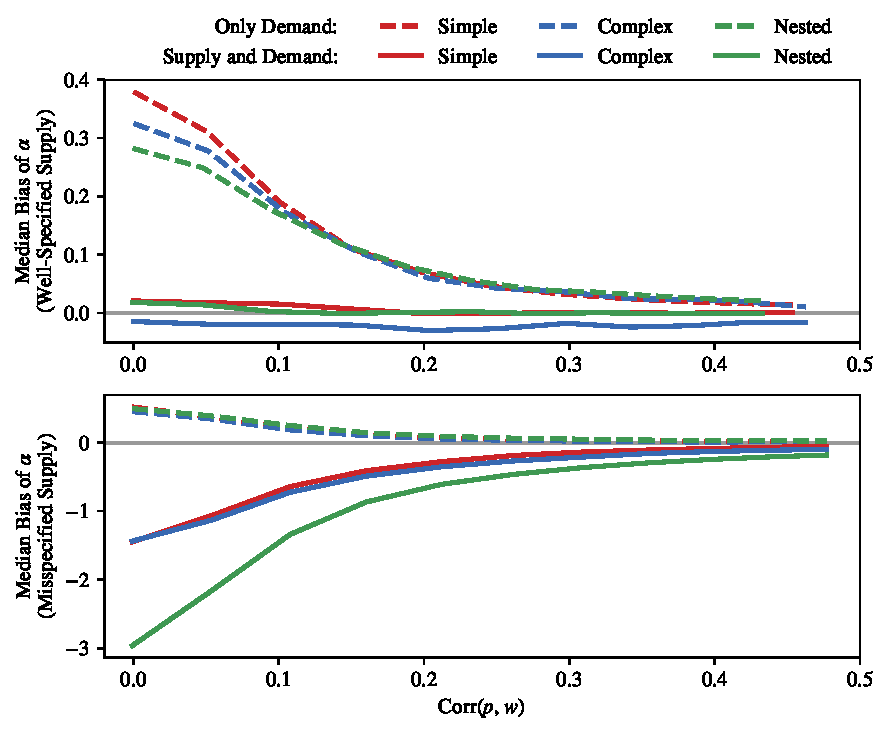
\includegraphics[height=0.95\textheight]{../demand/resources/strength_blp_approximate_bias_alpha_plot.pdf}
\end{center}
\end{frame}


\begin{frame}{What about Hausman Instruments?}
AKA contemporaneous prices of same product in a different market.
\begin{itemize}
    \item Idea is to pick up common cost shocks:
     $$p_{jmt} = c_{jmt} + \eta_{jmt}$$
     \item But this places strong assumptions on nature of demand shocks (and markups $ \eta_{jmt}$)
     \item Even with FE: $\xi_{jmt} = \xi_j + \xi_t + \underbrace{\Delta \xi_{jt}}_{=0} + \Delta \xi_{jmt}$
     \item A common complaint: national advertising might increase demand for a product in multiple geographic markets.
\end{itemize}
\end{frame}



\begin{frame}{Markup Shifters}
The equilibrium markup is a function of \alert{everything!} $\eta_{jt}(\mathbf{p},\mathbf{s},\xi_t,\omega_t,\textrm{x}_{t},\textrm{w}_{t},\textrm{v}_t,\textrm{y}_t,\theta_2)$:
\begin{itemize}
\item It is obviously \alert{endogenous} (depends on error terms)!
\item But lots of potential instruments beyond \alert{excluded} $\textrm{v}_t$ or $\textrm{w}_t$.
\item Idea: cross-market variation in number or strength of competitors
\begin{itemize}
\item Also $\textrm{v}_{-j}$ and $w_{-j}$ and $x_{-j}$.
\item Not $p_{-j}$ or $\xi_{-j}$, etc.
\item The idea is that these instruments shift the \alert{marginal revenue curve}.
\item What is a good choice of $f(x_{-j})$? etc.
\end{itemize}
\end{itemize}
\end{frame}




\begin{frame}{BLP Instruments}
\begin{itemize}
\item Common choices are average characteristics of other products in the same market $f(x_{-j,t})$. \alert{BLP instruments}
\begin{itemize}
\item Same firm $z_{1jt} = \overline{x}_{-j_f,t} = \frac{1}{\left\vert{F_j}\right\vert}  \sum_{k \in \mathcal{F}_j} x_{kt} - \frac{1}{\left\vert{F_j}\right\vert} x_{jt}$.
\item Other firms $z_{2jt}=\overline{x}_{\cdot t} - \overline{x}_{-j_f,t} - \frac{1}{J} x_{jt}$.
\item Plus regressors $(1, x_{jt})$.
\item Plus higher order interactions 
\end{itemize}
\item Technically linearly independent for large (finite) $J$, but becoming highly correlated.
\begin{itemize}
\item Can still exploit variation in number of products per market or number of products per firm.
\end{itemize}
\item Correlated moments $\rightarrow$ ``many instruments''.
\begin{itemize}
\item May be inclined to ``fix'' correlation in instrument matrix directly.
\end{itemize}
\end{itemize}
\end{frame}


% \begin{frame}{Armstrong (2016): Weak Instruments?}
% Consider the limit as $J \rightarrow \infty$
% \begin{eqnarray*}
% \frac{s_{jt}(\mathbf{p_t})}{\left|\frac{\partial s_{jt}(\mathbf{p_t})}{\partial p_{jt}}\right|} = \frac{1}{\alpha} \frac{1}{1-s_{jt}} \rightarrow \frac{1}{\alpha}
% \end{eqnarray*}
% \begin{itemize}
% \item Hard to use markup shifting instruments to instrument for a constant.
% \item How close to the constant do we get in practice?
% \item Average of $x_{-j}$ seems like an especially poor choice. Why?
% \item Shows there may still be some power in: products per market, products per firm.
% \item Convergence to constant extends to mixed logits (see Gabaix and Laibson 2004).
% \item Suggests that you really need cost shifters.
% \end{itemize}
% \end{frame}


\begin{frame}{Differentiation Instruments: Gandhi Houde (2019)}
\begin{itemize}
\item Also need instruments for the $\Sigma$ or $\sigma$ random coefficient parameters.
\item Instead of average of other characteristics $f(x) = \frac{1}{J-1} \sum_{k \neq j} x_k$, can transform as distance to $x_j$.
\begin{align*}
d_{jt} ^k=  |x_k - x_j |
\end{align*}
\item And use this transformed to construct two kinds of IV (Squared distance, and count of local competitors)
\begin{align*}
DIV_1 &= \sum_{j \in F}  d_{jt}^2,  \quad  \sum_{j \notin F}  d_{jt}^2 \\
DIV_2 &= \sum_{j \in F}  \mathbb{I}[d_{jt} < c]   \quad \sum_{j \notin F}   \mathbb{I}[d_{jt} < c]
\end{align*}
\item They choose $c$ to correspond to one standard deviation of $x$ across markets.
\item Monotonicity?
\end{itemize}
\end{frame}


% \begin{frame}{Differentiation Instruments: Gandhi Houde (2019)}
% \begin{center}
%  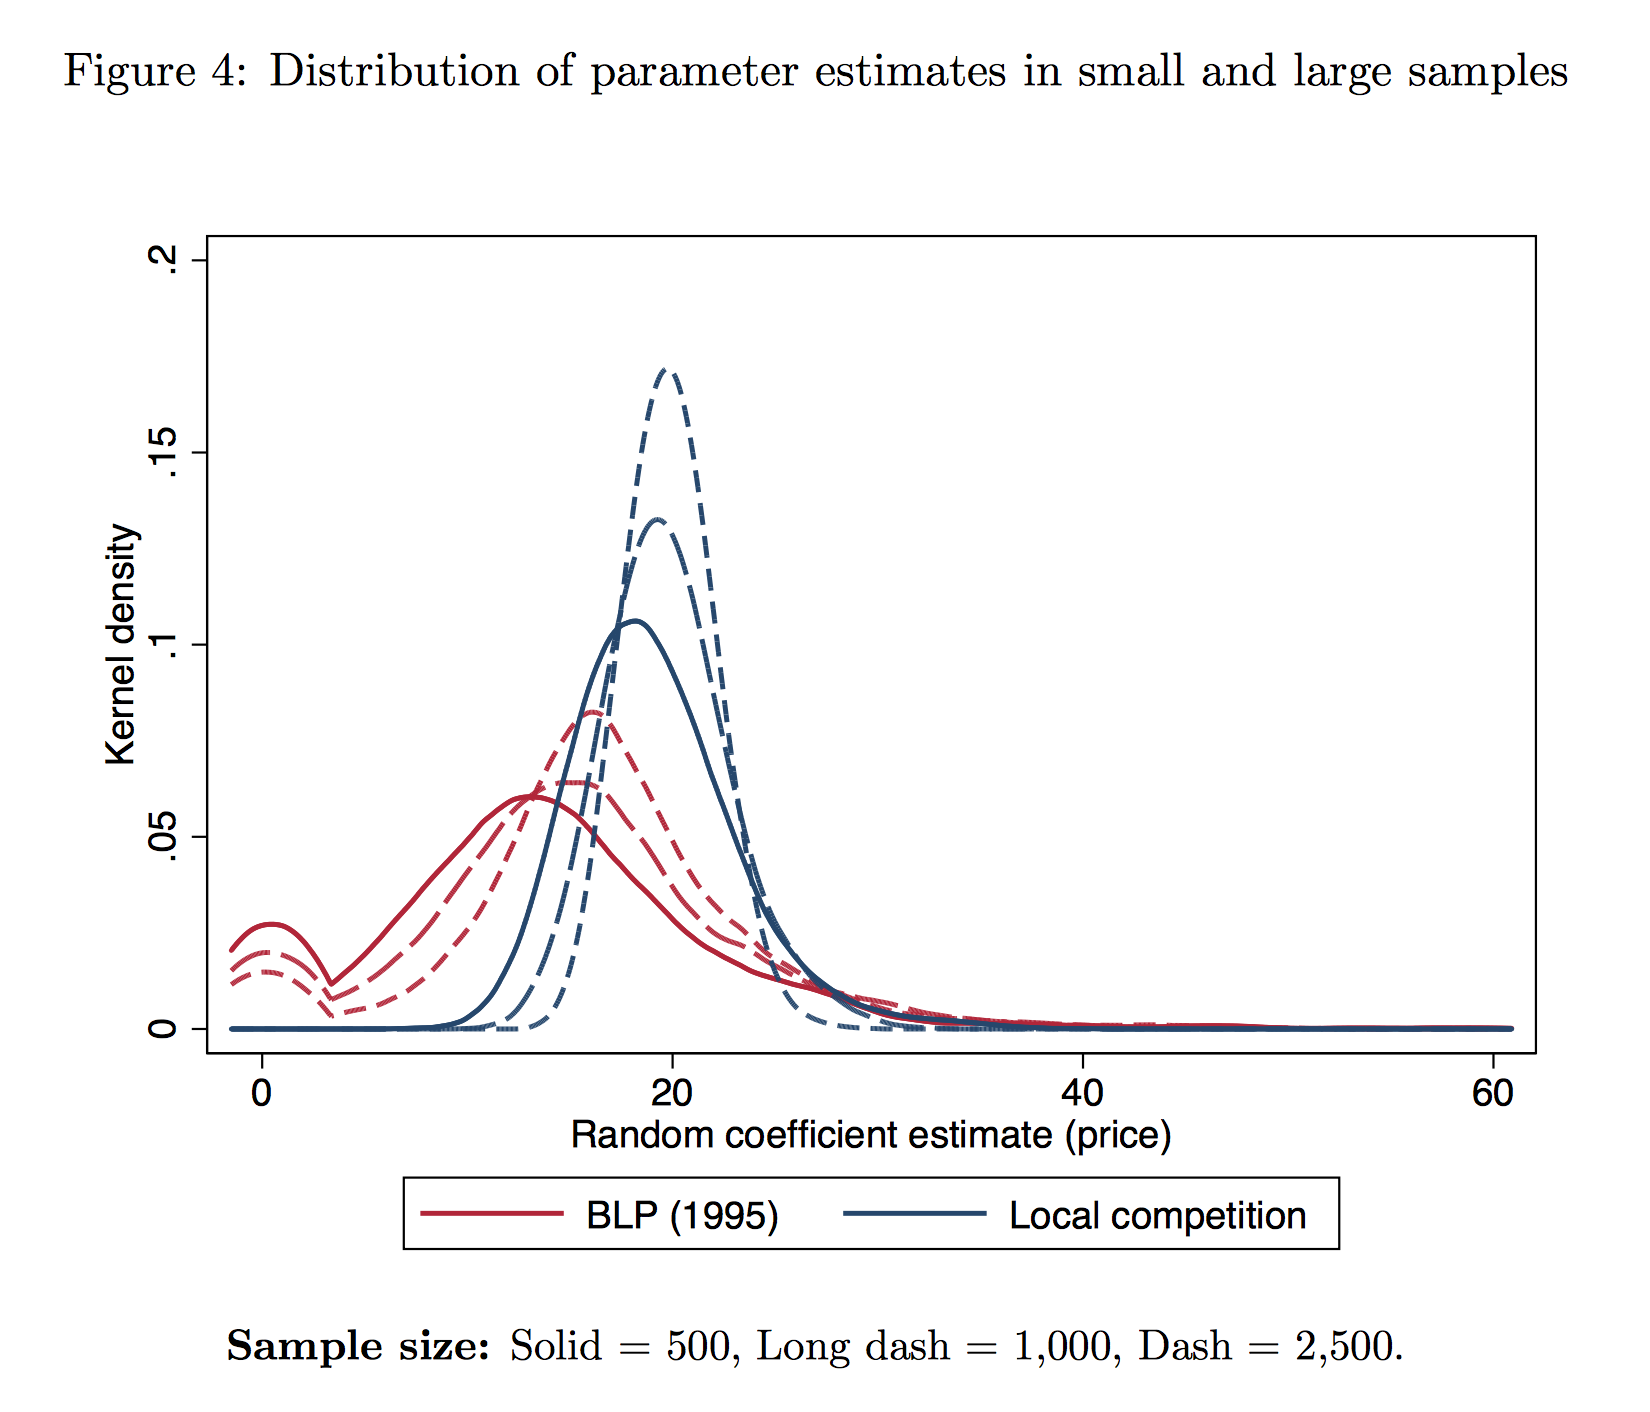
\includegraphics[height=0.9\textheight]{../demand/resources/d_iv1.png}
% \end{center}
% \end{frame}


% \begin{frame}{Intuition from Linear IV (FRAC: Salanie and Wolak)}
% Simple case where $\theta_0 = (\beta_0, \pi_0, \sigma_0)'$. A second-order Taylor expansion around $\pi_0 = \sigma_0 = 0$ gives the following linear model with four regressors:
% \begin{equation}
%     \label{eq:frac}
%     \log\frac{\mathcal{S}_{jt}}{\mathcal{S}_{0t}} \approx \beta_0 x_{jt} + \sigma_0^2 a_{jt} + \pi_0 m_t^y x_{jt} + \pi_0^2 v_t^y a_{jt} + \xi_{jt}, \quad a_{jt} = \Big(\frac{x_{jt}}{2} - \sum_{k \in \mathcal{J}_t} \mathcal{S}_{kt} \cdot x_{kt}\Big) \cdot x_{jt}
% \end{equation}
% \begin{itemize}
%     \item $m_t^y = \sum_{i \in \mathcal{I}_t} w_{it} \cdot y_{it}$ is the within-market demographic mean
%     \item $v_t^y = \sum_{i \in \mathcal{I}_t} w_{it} \cdot (y_{it} - m_t^y)^2$ is its variance
%     \item $a_{jt}$ is an ``artificial regressor'' that reflects within-market differentiation of the product characteristic $x_{jt}$.\\
%     \item Linear but we still need an IV for $a_{jt}$.
% \end{itemize}
% Implemented in Julia by Jimbo Brand  \url{https://github.com/jamesbrandecon/FRAC.jl}
% % where $m_t^y = \sum_{i \in \mathcal{I}_t} w_{it} \cdot y_{it}$ is the within-market demographic mean, $v_t^y = \sum_{i \in \mathcal{I}_t} w_{it} \cdot (y_{it} - m_t^y)^2$ is its variance, and $a_{jt}$ is an ``artificial regressor'' that reflects within-market differentiation of the product characteristic $x_{jt}$.\footnote{\cite{salanie2019fast} give additional intuition for the functional form of $a_{jt}$. A quadratic form is unsurprising because $x_{jt}$ multiplied $\nu_{it}$. The $\frac{1}{2}$ comes from the symmetric shape of the logistic distribution.} If $\pi_0 = \sigma_0 = 0$, the approximation is exact, and collapses to a simple logit regression: $\log(\mathcal{S}_{jt} / \mathcal{S}_{0t}) = \delta_{jt} = \beta_0 x_{jt} + \xi_{jt}$.
% \end{frame}


% \begin{frame}{Connection or when do GH IV work well?}
% Recall the GH IV are:
% \begin{align*}
% J \cdot x_{jt}^2 + \underbrace{\sum_k x_{kt}^2}_{\text{ constant for } t } - 2 \sum_k x_{jt} \cdot x_{kt}
% \end{align*}
% and the artificial regressor is
% \begin{align*}
% \frac{1}{2} x_{jt}^2 - 2 x_{jt} \cdot \sum_k \mathcal{S}_{kt}  \cdot x_{kt}
% \end{align*}
% \begin{itemize}
% \item We should be \alert{share weighting} the interaction term, but GH assume equal weighting.\\
% \item Should be able to do better than these IV (but ideal is infeasible...)
% \item Alternative take: GH propose IIA test that looks a lot like Salanie Wolak estimator. Good for starting values? Or as pre-test for heterogeneity?
% \item Warning: I find these are always nearly colinear and run PCA first...
% \end{itemize}
% \end{frame}


% \begin{frame}{Optimal Instruments}
% \begin{itemize}
% \item Since any $f(x,z)$ satisfies our orthogonality condition, we can try to choose $f(x,z)$ as a \alert{basis} to approximate optimal instruments. (Newey 1990)
% \item This is challenging in practice -- and in fact suffers from a curse of dimensionality.
% \item This is frequently given as a rationale behind higher order $x$'s.
% \item When the dimension of $x$ is low -- this may still be feasible. ($K \leq 3)$.
% \end{itemize}
% \end{frame}



% \begin{frame}{Optimal Instruments (Chamberlain 1987)}
% Chamberlain (1987) asks how can we choose $f(z_i)$ to obtain the semi-parametric efficiency bound with conditional moment restrictions:
% \begin{align*}
% \mathbb{E}[g(z_i,\theta) | z_i]=0 \Rightarrow \mathbb{E}[g(z_i,\theta) \cdot f(z_i) ]=0 
% \end{align*}
% Recall that the asymptotic GMM variance depends on $(G'\, \Omega^{-1} G\,)$

% The answer is to choose instruments related to the (expected) Jacobian of moment conditions w.r.t $\theta$. The true Jacobian at $\theta_0$ is \alert{infeasible}:
% \begin{align*}
% G=\mathbb{E}\left[\frac{\partial g(z_i,\theta)}{\partial \theta} | z_i, \theta_0 \right]
% \end{align*}
% %Dominguez and Lobato (2004) point out we can get unlucky and choose an $f(z_i)$ such that $\theta$ is no longer identified(!)
% \end{frame}


% \begin{frame}{Optimal Instruments (Chamberlain 1987)}
% Consider the simplest IV problem:
% \begin{align*}
% y_i &= \beta x_i + \gamma v_i + u_i \quad \text{ with } \quad \mathbb{E}[u_i | v_i, z_i] =0 \\
% u_i &= \left(y_i - \beta x_i - \gamma v_i \right) \\
% g(x_i,v_i,z_i) &= \left(y_i - \beta x_i - \gamma v_i \right) \cdot [v_i,\, z_i]
%  \end{align*}
%  Which gives:
% \begin{align*}
% \mathbb{E}\left[\frac{\partial g(x_i,v_i, z_i,\theta)}{\partial \gamma} \mid v_i, z_i \right] &\propto v_i\\
% \mathbb{E}\left[\frac{\partial g(x_i,v_i, z_i,\theta)}{\partial \beta} \mid v_i, z_i \right] &
% \propto \mathbb{E}\left[x_i \mid v_i, z_i \right]
% \end{align*}
% We can't just use $x_i$ (bc endogenous!), but you can also see where 2SLS comes from...
% \end{frame}




% \begin{frame}{Optimal Instruments (Newey 1990)}
% From previous slide, nothing says that $\mathbb{E}\left[x_i \mid v_i, z_i \right]$ needs to be \alert{linear}!
% \begin{itemize}
% \item Since any $f(x,z)$ satisfies our orthogonality condition, we can try to choose $f(x,z)$ as a \alert{basis} to approximate optimal instruments.
% \item Why? Well affine tranformations of instruments are still valid, and we span the same vector space!
% \item We are essentially relying on a non-parametric regression that we never run (but could!)
% \begin{itemize}
% \item This is challenging in practice -- and in fact suffers from a curse of dimensionality.
% \item This is frequently given as a rationale behind higher order $x$'s.
% \item When the dimension of $x$ is low -- this may still be feasible. ($K \leq 5)$.
% \item But recent improvements in sieves, LASSO, non-parametric regression are encouraging.
% \end{itemize}
% \end{itemize}
% \end{frame}





\begin{frame}{Takeaway}
What does this mean:
\begin{itemize}
    \item We should always check \alert{first stage} $\mathbb{E}[p \mid x, z]$ before we do anything else.
    \item May want to consider adding a supply side (if you're willing to assume for counterfactuals, why not?)
    \item Certainly should do \texttt{results.compute\_optimal\_instruments()} in PyBLP. (but you need a good first stage)
\end{itemize}
\end{frame}


\section{Some New Things}

\begin{frame}{Back to Diversion}
 Raise price of good $j$. People leave. What fraction of leavers switch to $k$?
\begin{eqnarray*}
D_{jk} (p_j,p_{-j})= \frac{\frac{\partial q_k}{\partial p_j}}{\left|\frac{\partial q_j}{\partial p_j} \right|}
\end{eqnarray*}
It's one of the best ways economists have to characterize competition among sellers.
\begin{itemize}
\item High Diversion: Close Substitutes $\rightarrow$ Mergers more likely to increase prices.
\item Very low diversion $\rightarrow$ products may not be in the same market.\\ (ie: Katz \& Shapiro). This is just hypothetical monopolist or SSNIP test.
\item Demand Derivatives NOT elasticities.
\item No equilibrium responses.
\end{itemize}
\end{frame}





\begin{frame}
\frametitle{Diversion: In Practice}
\begin{enumerate}
\item Calculated from an estimated demand system (ratio of estimated cross-price to own-price demand derivatives)
\item Consumer surveys (what would you buy if not this?)
\item Obtained in `course of business' (sales reps, internal reviews)
\end{enumerate}
Antitrust authorities may prefer different measures in different settings. Are they concerned about:
\begin{itemize}
\item Small but widespread price hikes?
\item Product discontinuations or changes to availability?
\end{itemize}
Is it sufficient to rely on data from merging firms only?
\begin{itemize}
\item Do we need diversion to other products in the `market' or other functions of market-level data?
\item Discrete-choice demand models imply that `aggregate diversion' (including to an outside good) sums to one.
\end{itemize}
\end{frame}


\begin{frame}{Diversion as Treatment Effects}
\begin{description}
\item[Outcome] $Y_i \in \{0,1\}$ denotes the event that consumer $i$ purchases product $k$: $d_{ik}(P_j)=1$.
\item[Treatment] $T_i \in \{0,1\}$ denotes the event that consumer $i$ does \textbf{not} purchase product $j$. In other words $T_i = 0$ implies $d_{ij}(P_j)=1$ and $T_i=1$ implies $d_{ij}(P_j)=0$.
\item[Instrument] $Z_i = P_j$ the price of $j$ induces consumers into not purchasing $j$.
\end{description}
\end{frame}



% \begin{frame}{Wald Estimator}
% The diversion ratio $D_{jk}(p_j,x) \equiv\frac{\partial q_k}{\partial P_j}(p_j,x)/-\frac{\partial q_j}{\partial P_j}(p_j,x)$ can be obtained as the limit of the Wald estimator where the price increase (or decrease) becomes small, so long as demand slopes \textit{strictly} downwards $\frac{\partial q_j}{\partial P_j} <0$.
% \begin{align*}                               
% \lim_{p_j' \rightarrow p_j} \frac{q_k(p_j',x) - q_k(p_j,x)}{-(q_j(p_j',x) - q_j(p_j,x))} \rightarrow \frac{\frac{\partial q_k}{\partial P_j}(p_j,x)}{-\frac{\partial q_j}{\partial P_j}(p_j,x)} \equiv D_{jk}(p_j,x)
% \end{align*}
% \end{frame}

\begin{frame}{Analogue to LATE Theorem Imbens Angrist (1994)}
\begin{theorem}[Conlon Mortimer (RJE 2021)]\ \\
\label{prop:late}
Under the following conditions:\\ 
(a) Mutually Exclusive and Exhaustive Discrete Choice: $d_{ij} \in \{0,1\}$ and $\sum_{j \in \mathcal{J}} d_{ij}=1$.\\
(b) Exclusion: $u_{ik}(p_j,x)=u_{ik}(p_j',x)$ for all $k \neq j$ and any $(p_j, p_j')$; \\
(c) Monotonicity: $u_{ij}(p_j',x) \leq u_{ij}(p_j,x)$ for all $i$ and any $(p_j' > p_{j})$; and \\
(d) Existence of a first-stage: $Pr(d_{ij}(p_j,x)=0) \neq Pr(d_{ij}(p_j',x)=0) $ for $(p_j' > p_{j})$; \\
(e) Random Assignment: $(u_{ij}(P_j,x),u_{ik}(P_j,x)) \perp P_j$. \\
\noindent
then the Wald estimator:
\begin{align*}
 \frac{q_k(p_j',x) - q_k(p_j,x)}{-\left(q_j(p_j',x) - q_j(p_j,x)\right)}=\mathbb{E}[D_{jk,i}(x) | d_{ij}(p_j,x) > d_{ij}(p_j',x)]
\end{align*}
\end{theorem}
\end{frame}

\begin{frame}{Diversion as MTE}
\footnotesize
What can we learn from a change in $p_j$?
\begin{align*}
 \frac{q_k(p_j',x) - q_k(p_j,x)}{-\left(q_j(p_j',x) - q_j(p_j,x)\right)}&=\mathbb{E}[D_{jk,i}(x) | d_{ij}(p_j,x) > d_{ij}(p_j',x)]\\
&= \int D_{jk,i}(x) \, w_i(z_j,z_j',x)  \, \partial F_i \quad \mbox{ with } w_i(z_j,z_j',x) = \frac{q_{ij}(z_j,x)- q_{ij}(z_j',x) }{q_j(z_j,x)- q_j(z_j',x)}
\end{align*}
\begin{itemize}
\item Individual diversion ratios in logit family are $D_{jk,i} = \frac{s_{ik}}{1-s_{ij}}$ and don't depend on $p_j,z_j$
\item Which individuals respond to $z_j$ or $p_j$ determines the weighting scheme only.
\end{itemize}
\end{frame}

\begin{frame}{Weights}
Again $D_{jk,i} = \frac{s_{ik}}{1-s_{ij}}$ for logit family and plain logit $D_{jk,i} = \frac{s_{k}}{1-s_{j}}$ for all $i$ and weights don't matter!
\begin{align*}
\int D_{jk,i}(x) \, w_i(z_j,z_j',x)  \, \partial F_i 
\end{align*}
\begin{center}
\begin{tabular}{rcc} 
& $w_i(z_j,z_j',x) \propto$ \\
\midrule second choice data & $s_{i j}(x)$ \\
price change $\frac{\partial}{\partial p_{j}}$ & $s_{i j}(x) \cdot\left(1-s_{i j}(x)\right) \cdot\left|\alpha_{i}\right|$ \\
characteristic change $\frac{\partial}{\partial x_{j}}$ & $s_{i j}(x) \cdot\left(1-s_{i j}(x)\right) \cdot\left|\beta_{i}\right|$ \\
small quality change $\frac{\partial}{\partial \xi_{j}}$ & $s_{i j}(x) \cdot\left(1-s_{i j}(x)\right)$ \\
\midrule
\end{tabular}\\
\end{center}
\end{frame}

\section{A Useful (?) Extension (Conlon, Mortimer, Sarkis 2023)}




\begin{frame}{Definitions: Second Choices}
For any (semiparametric) mixture of logits we can write the probability that individual $i$ chooses $k$ as their \alert{second choice} given that $j$ is their first choice as:
\begin{align*}
D_{j \rightarrow k} & \equiv \mathbb{P}(\text{ chooses } k \in \mathcal{J} \setminus \{j\} \mid
\text{ chooses } j \in \mathcal{J} )\\
&= \sum_{i=1}^I \pi_i \cdot \frac{s_{ik}}{1-s_{ik}} \cdot \frac{s_{ij}}{s_j}
\end{align*}
It is convenient to interpret $D_{j \rightarrow k}$ as the $(j,k)$th entry in the second-choice matrix $\mathbf{D}(\mathbf{S},\pi)$.
\end{frame}




\begin{frame}{Our Semiparametric Problem}
\small
\begin{align*}
\min _{(\mathbf{S}, \pi) \geq 0} \left\|\mathcal{P}_{\Omega}(\mathcal{D}-\mathbf{D}(\mathbf{S},\pi))\right\|_{\ell_2}  &+ \lambda \left\|\mathcal{S}- \mathbf{S}\,\pi \right\|_{\ell_2} \text { with } \left\|\pi  \right\|_{\ell_1} \leq 1, \quad   \left\|\mathbf{s_i}  \right\|_{\ell_1} \leq 1.
\end{align*}
\vspace{-.25cm}
\begin{itemize}
    \item Constraints: Choice probabilities $s_{ij}$ sum to one, type weights $\pi_i$ sum to one.
\item Use cross validation to select \# of types $I$ and Lagrange multiplier $\lambda$.
\item Not-convex but not very difficult either.
\item $\ell_1$ constraints lead to \alert{sparsity}.
\item Goal: estimate $\mathbf{s_i}$ (choice probabilities) and corresponding weights $\pi_i$ (Finite Mixture)
\item Can also match \alert{price cost margins}
% \item Weights $\widetilde c_j$ and $c_j$ are proportional to $\ln q_j$
\end{itemize}
Would this be useful to folks at CMA?
\end{frame}



\begin{frame}{Second Choice Matrix}
\begin{itemize}
\item Individual $i$'s share for each choice given by $\mathbf{s_i} = [s_{i0},s_{i1},\ldots,s_{iJ}]$.
\item Aggregate shares by $\sum_{i=1}^I  \pi_i \cdot \mathbf{s_i} =\mathbf{s}$.
\item The matrix of individual diversion ratios is given by
$\mathbf{D}_i  = \mathbf{s_i}  \cdot \left[\frac{1}{(1-\mathbf{s_i})} \right]^T$. 
\end{itemize}
We write the $(J+1)\times (J+1)$ matrix of second-choice probabilities as:
\begin{align*}
\nonumber \mathbf{D} &=  \left(\sum_{i=1}^I \pi_i \cdot \mathbf{s_i} \cdot \left[\frac{1}{(1-\mathbf{s_i})} \right]^T \cdot \text{diag}(\mathbf{s_i}/\mathbf{s})^{-1}\right)^T \\
&=\text{diag}(\mathbf{s})^{-1}  \cdot \left(\sum_{i=1}^I \pi_i \cdot  \left[\frac{\mathbf{s_i}}{(1-\mathbf{s_i})} \right]\cdot  \mathbf{s_i}^T   \right) 
\end{align*}
\end{frame}

\begin{frame}{Second Choice Matrix: Continued}
Under relatively general conditions, second-choice probabilities can be written as:
\begin{align*}
\mathbf{D}= \text{diag}(\mathbf{s})^{-1}  \cdot  \left(\sum_{i=1}^I \pi_i\cdot 
\left[
\begin{array}{l}
\mid \\
\mathbf{s_i} \\
\mid
\end{array}\right] \cdot \left[\begin{array}{lll}
\horzbar  &\frac{\mathbf{s_i}}{1-\mathbf{s_i}}  & \horzbar
\end{array}\right] \right)
\end{align*}
\begin{itemize}
    \item Each individual diversion ratio is of rank one since it is the outer product of $\mathbf{s_i}$ with itself (and some diagonal ``weights'').
    \item The (unrestricted) matrix of diversion ratios $\mathbf{D}$ is $(J+1)\times(J+1)$.
    \item Logit restricts $\mathbf{D}$ to be of rank one. Nested logit of rank $\leq G$ (the number of non-singleton nests). Mixed logit to $\text{rank}(\mathbf{D})\leq I$ (but bound is likely uninformative).
\end{itemize}
In practice this works shockingly well (with some caveats).
\end{frame}







\appendix

\begin{frame}[plain,allowframebreaks,noframenumbering]{References}
    \bibliography{references}
\end{frame}


\end{document}